\documentclass{beamer}
\usepackage[utf8]{inputenc}
\usepackage{xcolor}
\usepackage{listings}
\usepackage{graphicx}
\usetheme[secheader]{Boadilla}
\definecolor{coultitre}{rgb}{0,0.65,0}
\setbeamercolor{structure}{fg=coultitre, bg=coultitre!40} 


\title{Vidéo surveillance, Streaming vidéo et contrôle de caméra via Android }
\author{Jérôme NAHELOU, Quentin NEBOUT, Romain SOLVE,\\Fabien QUINTARD}
\institute{\large{Chargé de Projet : Yérom-David Bromberg}\\ \bigskip{}
\small{Université Bordeaux 1}}
\date{29 mars 2011}

\begin{document}
\frame[plain]{
\includegraphics[scale=0.20]{logo-bdx1.pdf}\titlepage}

\AtBeginSection[]{
\begin{frame}<beamer>
\frametitle{Plan}
\small{\tableofcontents[currentsection,hideallsubsections]}
\end{frame}}

\begin{frame}
\frametitle{Plan de l'exposé}
\small{\tableofcontents[hideallsubsections]}
\end{frame}



\section{Aspect général de l'application}
  \subsection{Description}
  \begin{frame}
   \frametitle{Description de l'application}
   \begin{itemize}
   \item Fonctionnement sous Android
       \begin{itemize}
    	\item Téléphone mobile
   		\item Tablette tactile
    	\end{itemize}
   \item Réservée aux caméras de la marque Axis
   		\begin{itemize}
    	\item Compatible pour tous les modèles
   		\item Intègration des fonctions propres aux caméras
    	\end{itemize}
   \item Facilité d'utilisation
   		\begin{itemize}
    	\item Sauvegarde du profil utilisateur
   		\item Contrôle tactile
    	\end{itemize}
   \end{itemize}
  \end{frame}



\subsection{Besoins}
  \begin{frame}
   \frametitle{Besoins pour l'application}

  \centering
  \begin{minipage}{0.95\textwidth}
	\begin{itemize}
    \item Besoins fonctionels de l'application
    \end{itemize}
    \end{minipage}
   
     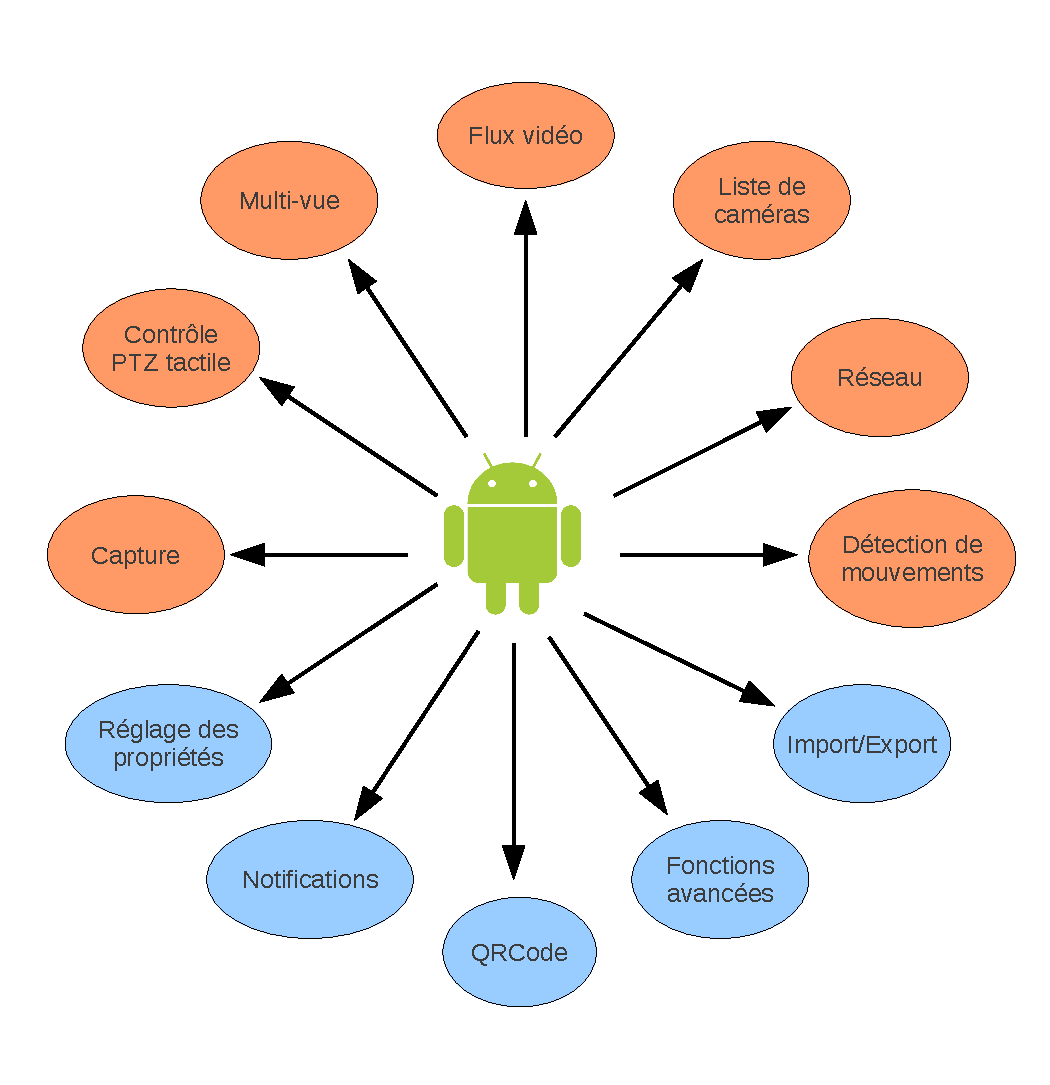
\includegraphics[scale=0.4]{Images/besoinsF.pdf}
   
  \end{frame}

\subsection{Besoins}
  \begin{frame}
   \frametitle{Besoins pour l'application}

  \centering
  \begin{minipage}{0.95\textwidth}
	\begin{itemize}
    \item Besoins non fonctionels de l'application
    \end{itemize}
    \end{minipage}
   
     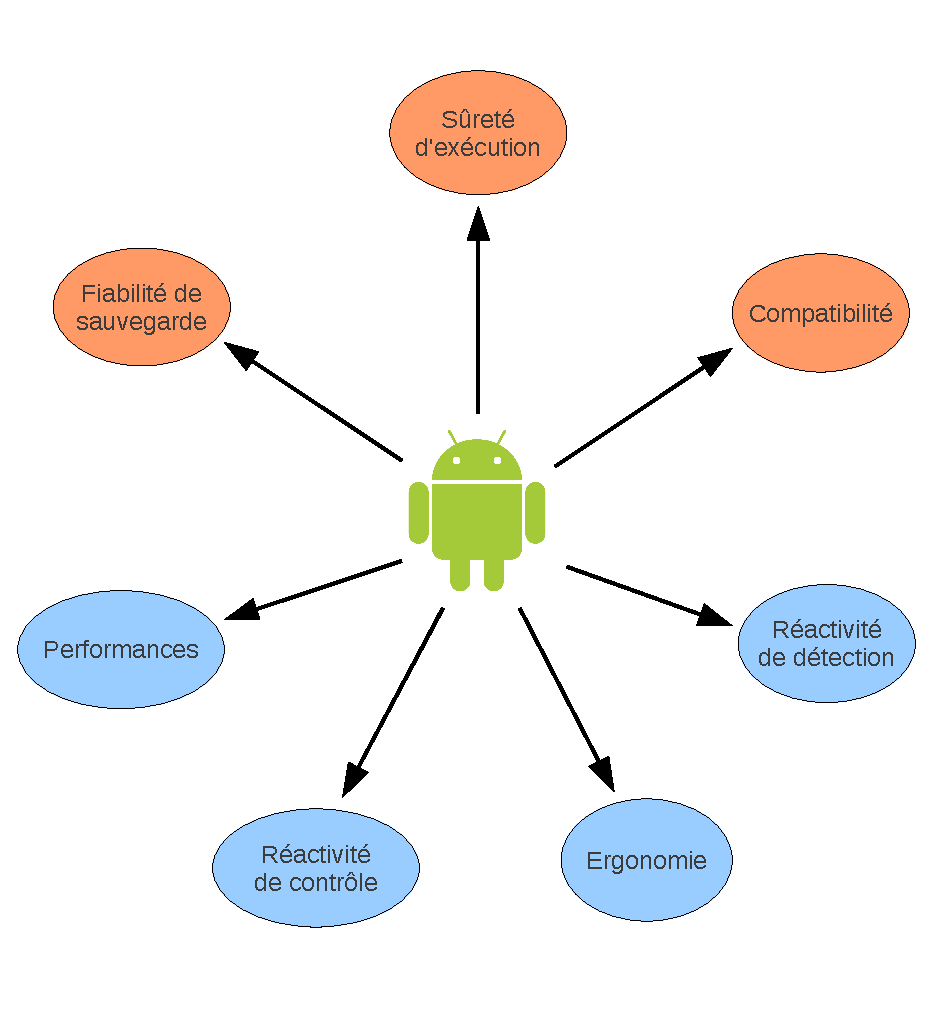
\includegraphics[scale=0.4]{Images/besoinsNF.pdf}
   
  \end{frame}

\section{Gestion des caméras}
  \begin{frame}
   \frametitle{Gestion des caméras}


\begin{figure}[H]
  \centering
  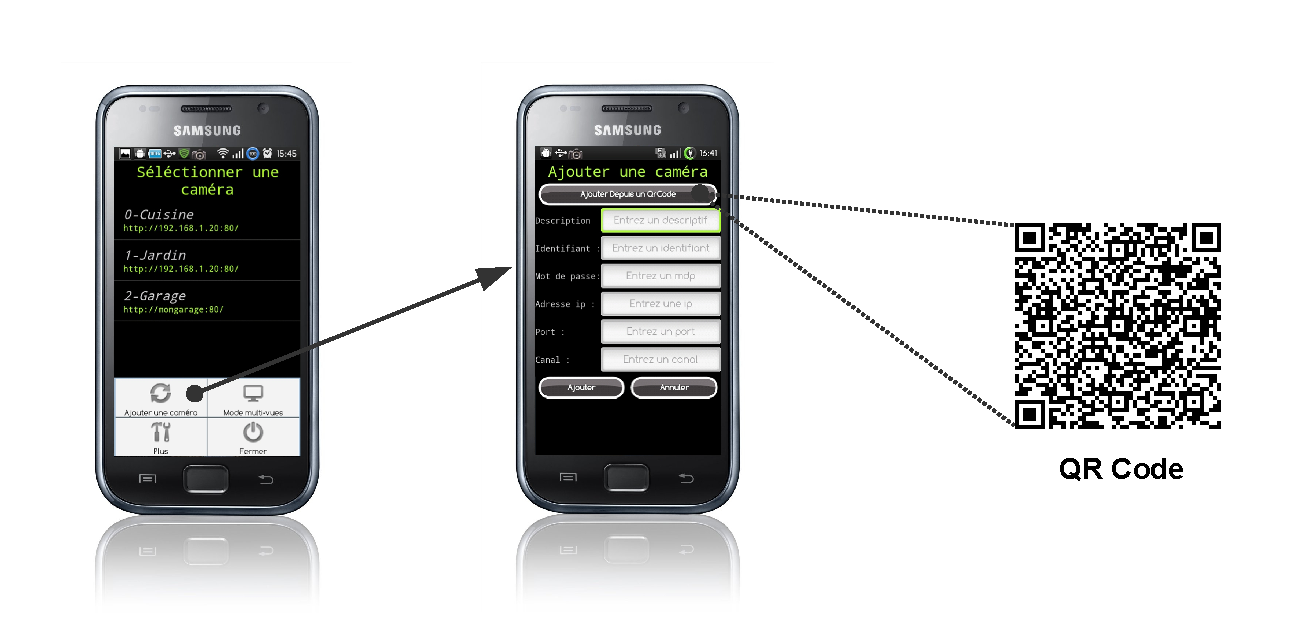
\includegraphics[scale=0.25]{Images/ImageSlide5.pdf}
     \begin{itemize}
    \item Ecran d'accueil de l'application, accès aux différentes activités
    \item Liste illimitée de caméras sauvegardable
    \item Gestion complète des caméras : ajout / édition / suppression
    \item Possiblité d'ajout par QRCode
   \end{itemize}
  \end{figure}  

  \end{frame}


\section{Simple vue}
  \begin{frame}
   \frametitle{Simple vue}


\begin{figure}[H]
  \centering
     \begin{enumerate}
    \item Visualisation de base (contrôle PTZ tactile)
    \item Interface de contrôles avancés
    \item Mode détection de mouvements
   \end{enumerate}
   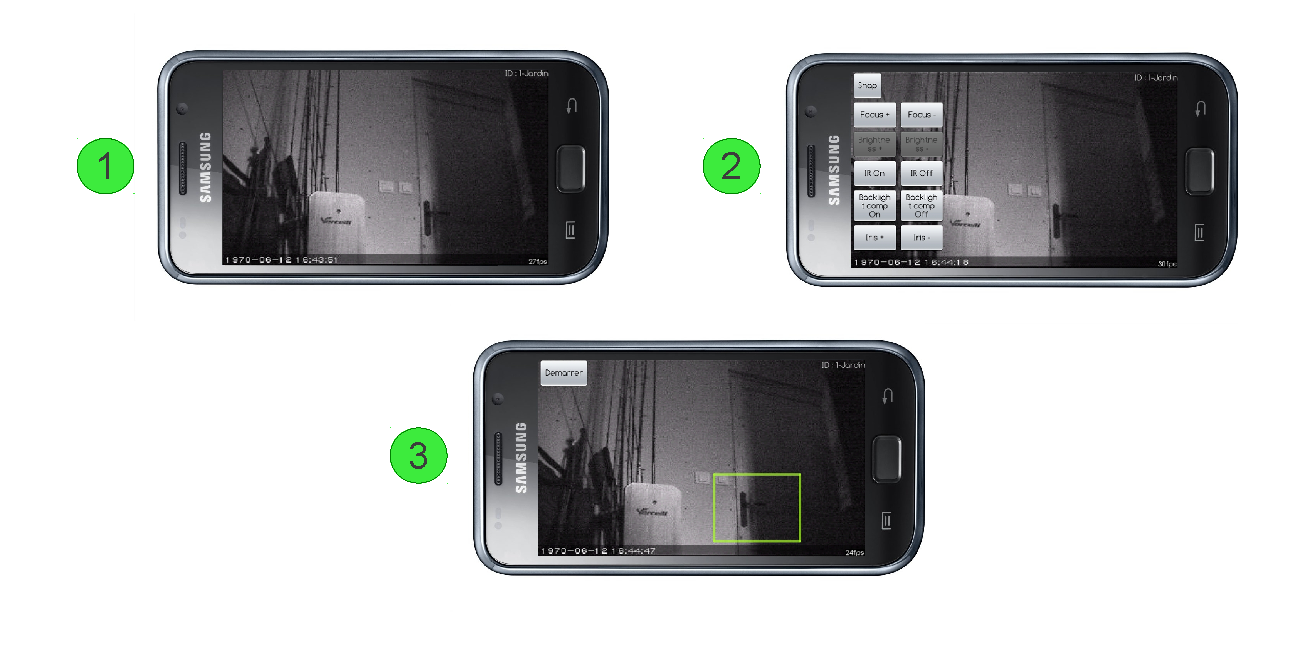
\includegraphics[scale=0.25]{Images/ImageSlide6.pdf}
  \end{figure}  

  \end{frame}

\subsection{Communication avec la caméra}
  \begin{frame}
   \frametitle{Communication et configuration}

  \begin{minipage}{0.94\textwidth}
  \centering
     \begin{itemize}
    \item Classe dédiée au traitement des requêtes HTTP envoyées à la caméra
    \begin{itemize}
      \item Codes réponses divers
      \item Parsage si nécessaire
      \newline
    \end{itemize}
    \item Chargement de la configuration et des fonctionnalités supportées
    \begin{itemize}
      \item PTZ, focus, iris, luminosité, \ldots
      \item Mode auto, résolutions d'images
      \item Audio, détection de mouvements
      \newline
    \end{itemize}
    \item Adaptation de l'interface aux différents modèles de caméra Axis
    \begin{itemize}
      \item Etat des boutons
      \item Choix de la résolution pour la capture
      \newline
    \end{itemize}
   	\end{itemize}
  \end{minipage}

  \end{frame}


\section{Contrôle PTZ tactile}
  \begin{frame}
   \frametitle{Contrôle PTZ tactile}


\begin{figure}[H]
  \centering
    \begin{itemize}
      \item Gestion du déplacement de la caméra (Pan/Tilt) avec 1 pointeur
      (1)
      \item Gestion du zoom avec 2 pointeurs (2)
      \item Réglage de la sensibilité dans les paramètres
   	\end{itemize}
   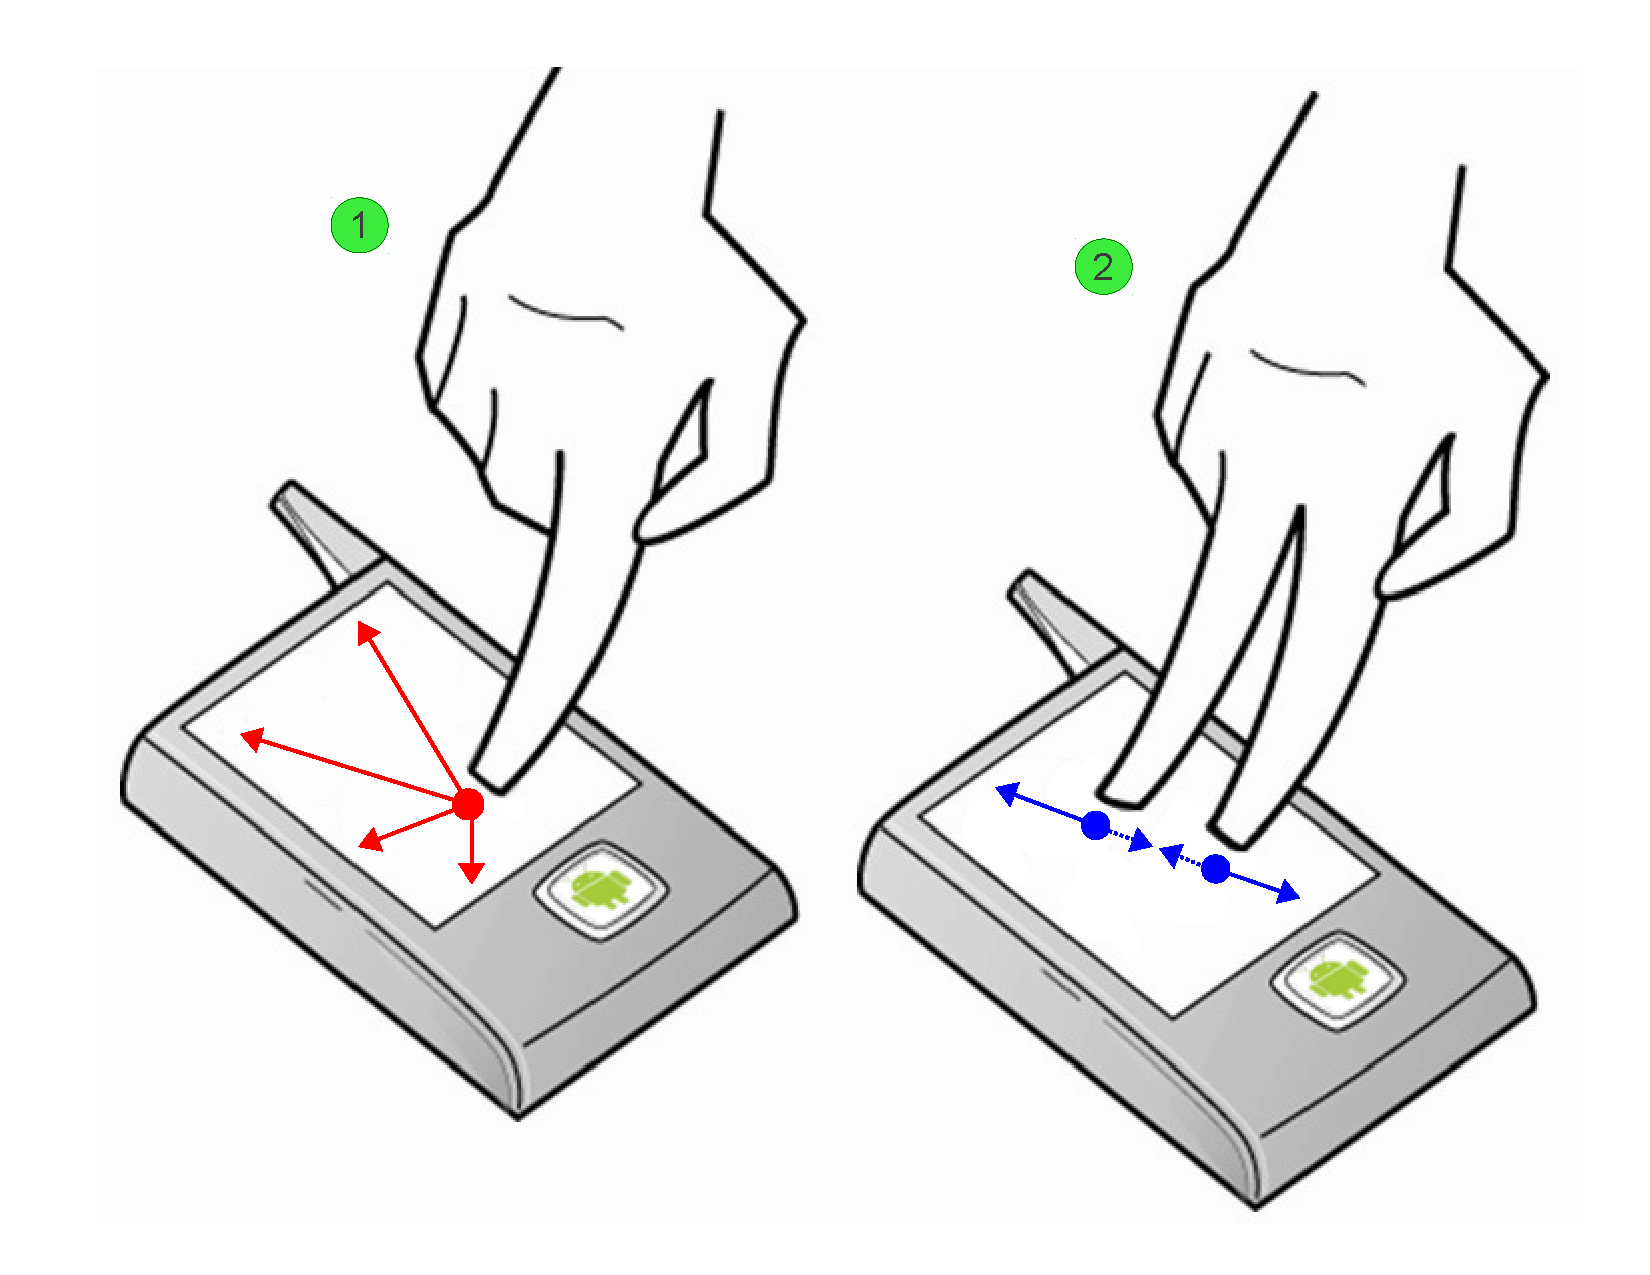
\includegraphics[scale=0.25]{Images/ImageSlide8.pdf}
  \end{figure}  

  \end{frame}


\section{Vue Multiple}
  \subsection{Analyse du besoin}
  \begin{frame}
   \frametitle{Analyse du besoin}


\begin{figure}[H]
  \centering
  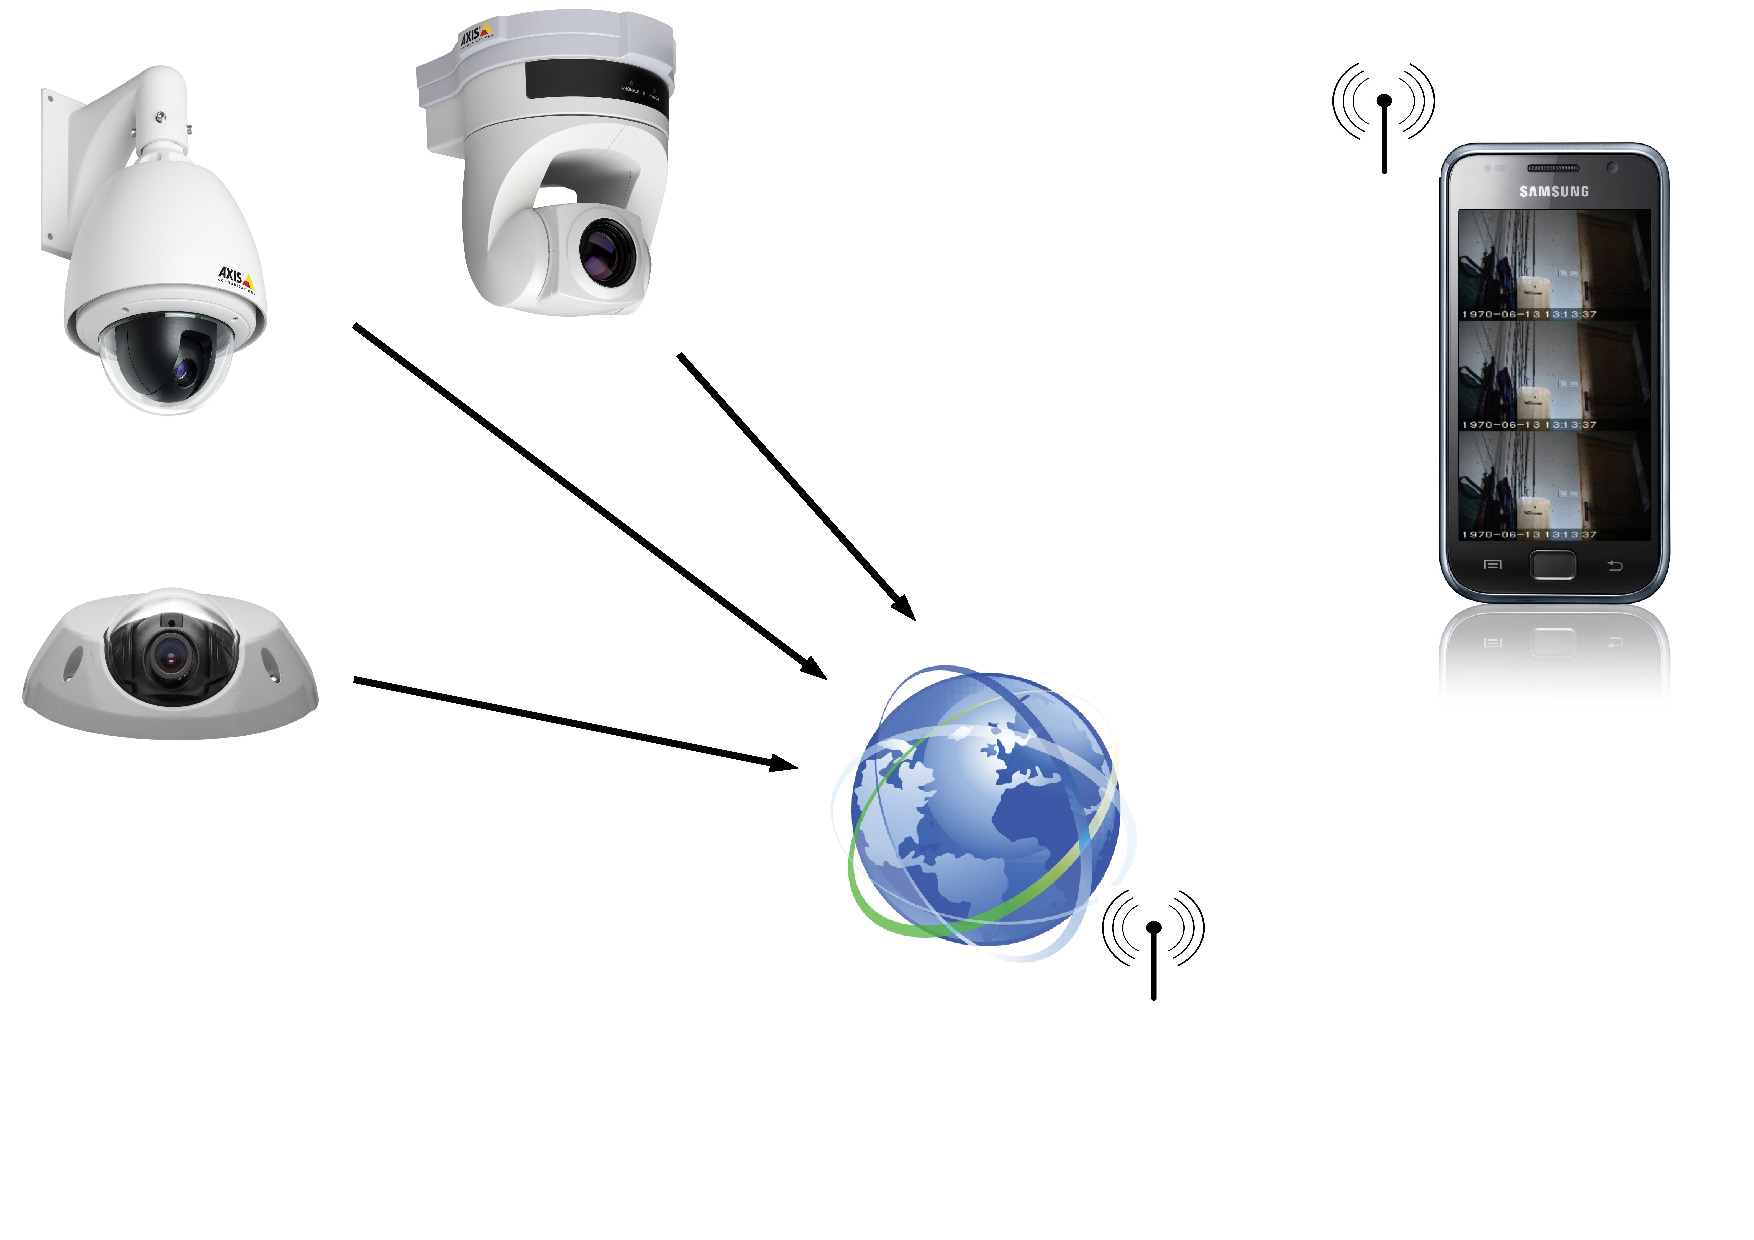
\includegraphics[scale=0.25]{Images/ImageSlide9.pdf}
     \begin{itemize}
    \item Possibilité de visionner 1 à 6 Caméras simultanément
    \item Choix de la disposition des caméras par l'utilisateur
    \item Réglage du nombre d'images par seconde
    \item Switch ``Multiple-Vue" - ``Vue unitaire"
   \end{itemize}
  \end{figure}  

  \end{frame}

  \subsection{Implémentation}
  \begin{frame}
   \frametitle{Implémentation}




  \end{frame}


\section{Détection de mouvement}
 \subsection{Analyse du besoin}
  \begin{frame}
   \frametitle{Détection des mouvements :}



\begin{columns}
\begin{column}{5cm}

   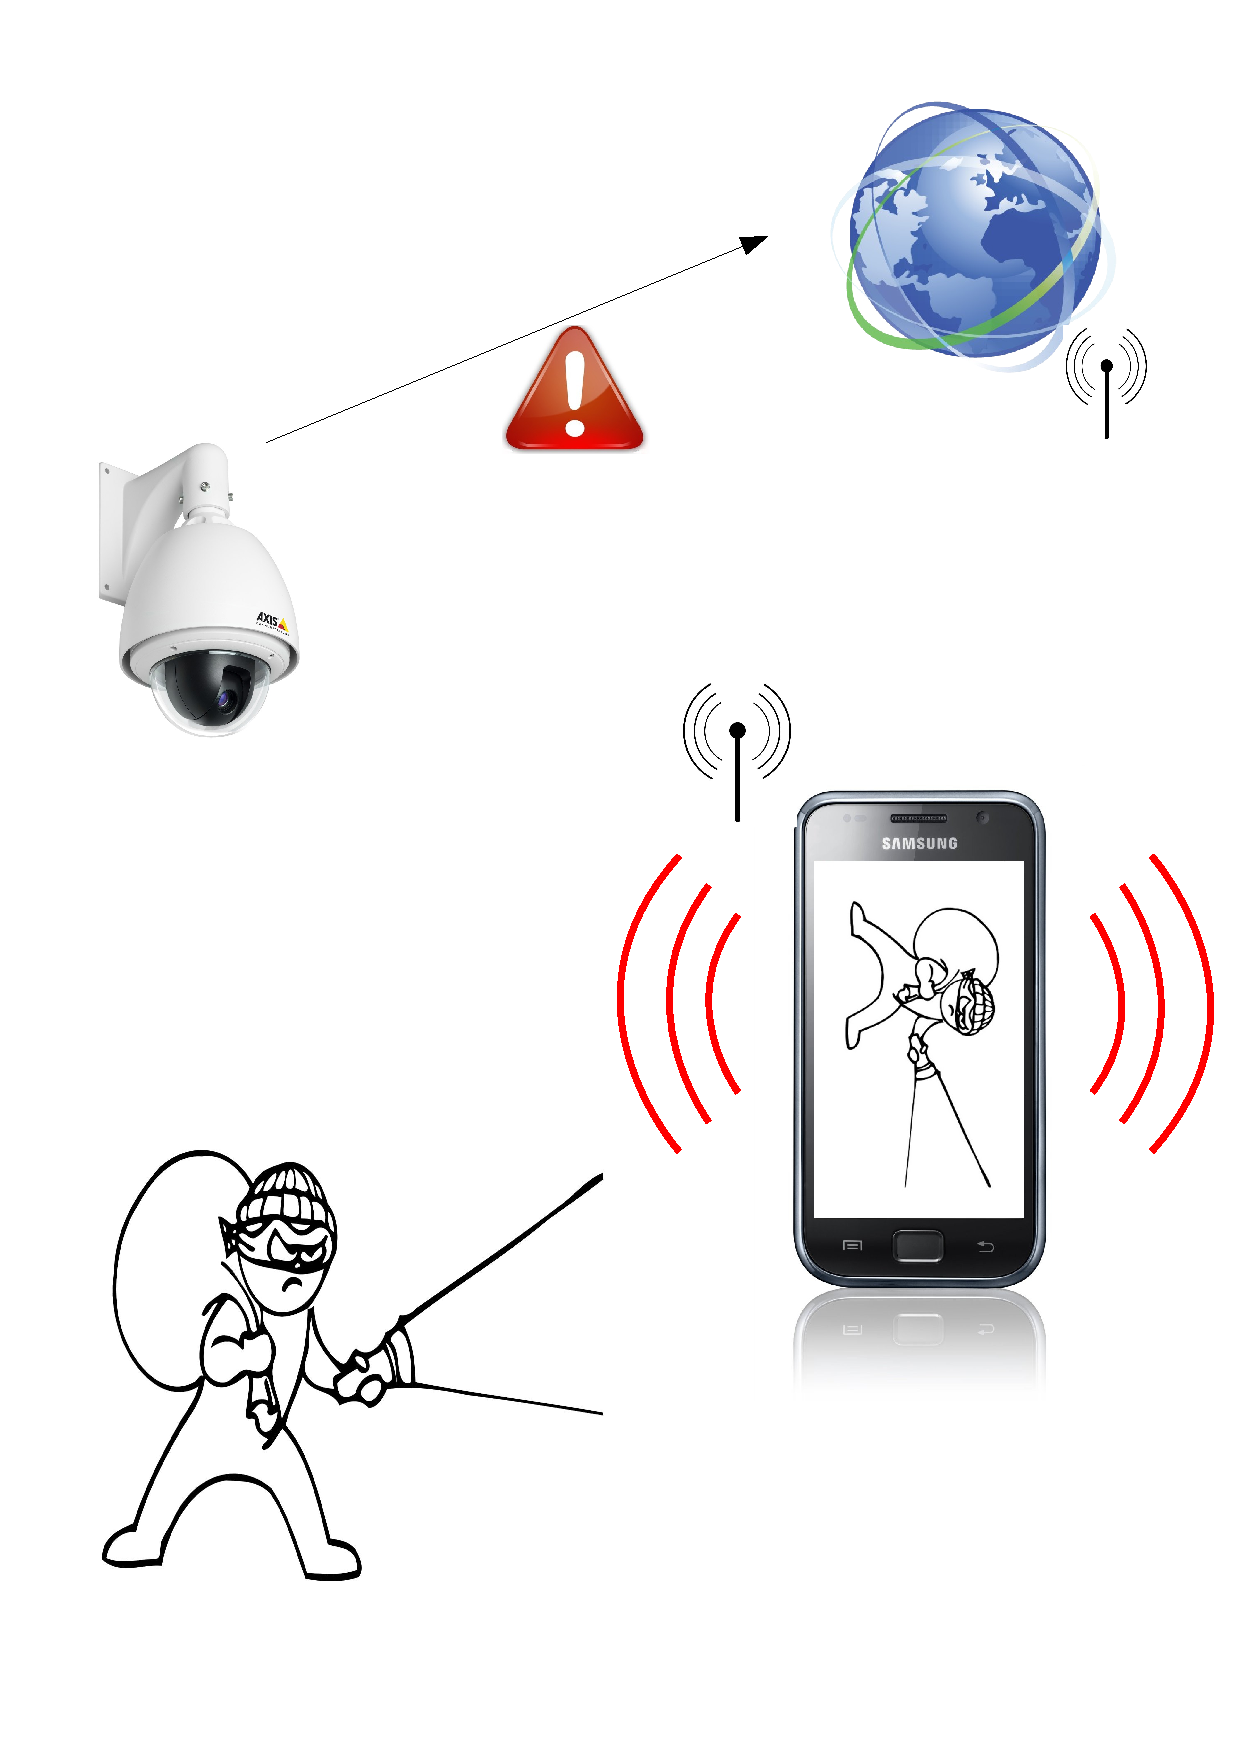
\includegraphics[scale=0.25]{Images/ImageSlide10.pdf}
\end{column}
\begin{column}{7cm}
\textbf{\textit{Caractéristiques :}} 
\begin{itemize}
    \item Réglage de la fenètre et du seuil de détection.
  	\item 1 à 10 fenètres par caméra.
  	\item Détection illimitée pour des caméras differente.
 	\item Notification via Vibration et Cliché instantanné.
 	\item Utilisation facile et intuitive.
\end{itemize}
\end{column}
\end{columns}
  \end{frame}

  \subsection{Implémentation}
  \begin{frame}
   \frametitle{Implémentation}

  \end{frame}

  
\subsection{Extras}
\begin{frame}
\frametitle{Extras}
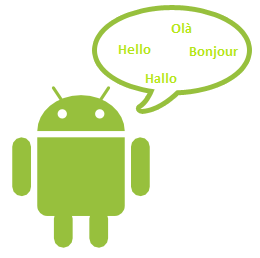
\includegraphics[width=3cm, height=2.5cm]{Images/ImageSlide11-3.png}\\
\begin{minipage}{0.69\textwidth}
\begin{itemize}
  \item Application Multi-langues
  \item Astuces au démarrage
  \item Snapshot
  \item Partage de l'application et des caméras
  \item Import-export de la configuration
\end{itemize}
\end{minipage}
\begin{minipage}{0.29\textwidth}
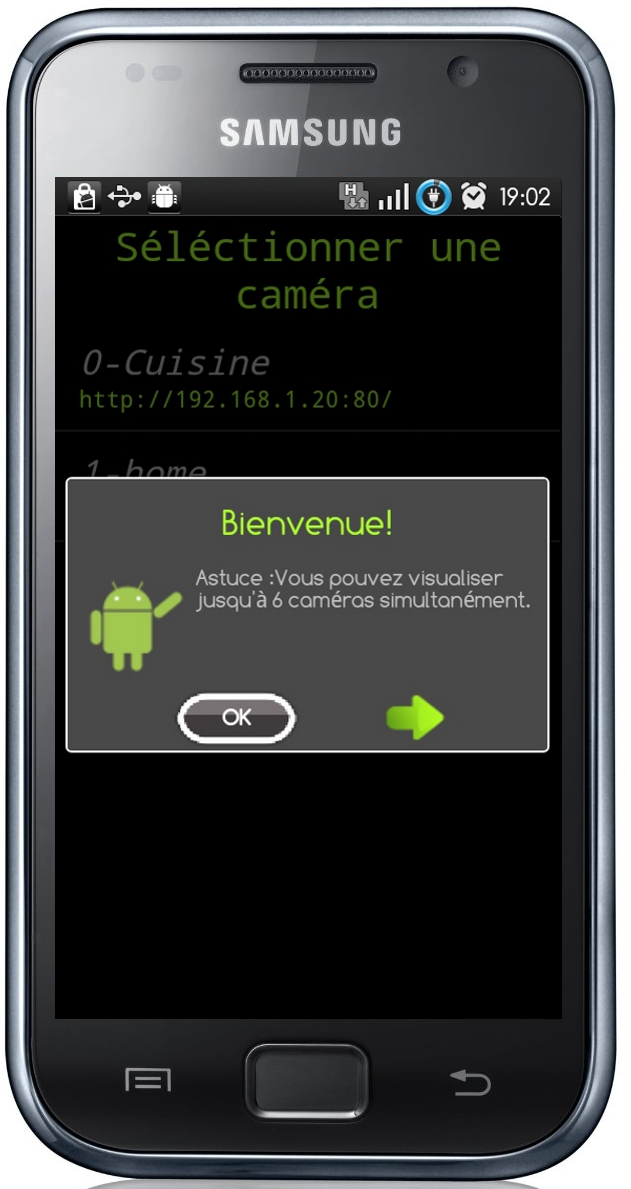
\includegraphics[width=2.5cm, height=4.5cm]{Images/ImageSlide11-3a.png}
\end{minipage}
\end{frame}
\section{Tests Unitaires}
\subsection{Principe}
  \begin{frame}
\begin{minipage}{0.59\textwidth}
\frametitle{Tests Unitaires}
Rôle des tests unitaires
  \begin{itemize}
 \item Garantir le bon fonctionnement de l'application
    \item Vérifier si les fonctions terminent bien
    \item Identifier étape par étape les erreurs éventuelles
\end{itemize} 
\end{minipage}
\begin{minipage}{0.39\textwidth}
 
\includegraphics[width=4cm, height=3.2cm]{Images/ImageSlide12.png}
\end{minipage}
\end{frame}
\subsection{Tests en réel}
 \begin{frame}
\begin{minipage}{0.59\textwidth}
   \frametitle{Tests en réel}
\begin{itemize}
    \item Suivi de l'exécution en continu avec le LogCat d'Android
    \item Utilisation intensive de 3 téléphones de marques différentes
    \item Tests sur une caméra Axis PTZ 214 avec l'ensemble des
    fonctionnalités implémentées
   \end{itemize}
\end{minipage}
\begin{minipage}{0.39\textwidth}
 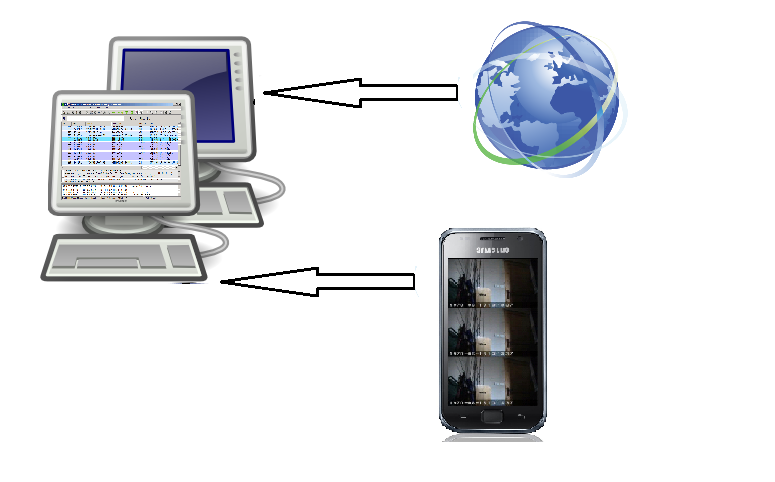
\includegraphics[width=4cm, height=3cm]{Images/ImageSlide13.png}
\end{minipage}
\end{frame}
  \begin{frame}
   \frametitle{Conclusion}
 \begin{itemize}
    \item Cahier des charges : Absence de son
    \item Application testée et opérationnelle
   \end{itemize}
   \begin{figure}[H]
    \centering
\includegraphics[width=2cm, height=2cm]{Images/ImageSlide14.png}
    \end{figure}
\end{frame}


\end{document}